% Generated by Sphinx.
\def\sphinxdocclass{report}
\documentclass[letterpaper,10pt,english]{sphinxmanual}
\usepackage[utf8]{inputenc}
\DeclareUnicodeCharacter{00A0}{\nobreakspace}
\usepackage{cmap}
\usepackage[T1]{fontenc}
\usepackage{babel}
\usepackage{times}
\usepackage[Bjarne]{fncychap}
\usepackage{longtable}
\usepackage{sphinx}
\usepackage{multirow}


\title{ThePythonGameBook Documentation}
\date{April 27, 2014}
\release{0.4}
\author{Horst JENS}
\newcommand{\sphinxlogo}{}
\renewcommand{\releasename}{Release}
\makeindex

\makeatletter
\def\PYG@reset{\let\PYG@it=\relax \let\PYG@bf=\relax%
    \let\PYG@ul=\relax \let\PYG@tc=\relax%
    \let\PYG@bc=\relax \let\PYG@ff=\relax}
\def\PYG@tok#1{\csname PYG@tok@#1\endcsname}
\def\PYG@toks#1+{\ifx\relax#1\empty\else%
    \PYG@tok{#1}\expandafter\PYG@toks\fi}
\def\PYG@do#1{\PYG@bc{\PYG@tc{\PYG@ul{%
    \PYG@it{\PYG@bf{\PYG@ff{#1}}}}}}}
\def\PYG#1#2{\PYG@reset\PYG@toks#1+\relax+\PYG@do{#2}}

\expandafter\def\csname PYG@tok@kt\endcsname{\def\PYG@tc##1{\textcolor[rgb]{0.56,0.13,0.00}{##1}}}
\expandafter\def\csname PYG@tok@mo\endcsname{\def\PYG@tc##1{\textcolor[rgb]{0.13,0.50,0.31}{##1}}}
\expandafter\def\csname PYG@tok@nd\endcsname{\let\PYG@bf=\textbf\def\PYG@tc##1{\textcolor[rgb]{0.33,0.33,0.33}{##1}}}
\expandafter\def\csname PYG@tok@sd\endcsname{\let\PYG@it=\textit\def\PYG@tc##1{\textcolor[rgb]{0.25,0.44,0.63}{##1}}}
\expandafter\def\csname PYG@tok@s\endcsname{\def\PYG@tc##1{\textcolor[rgb]{0.25,0.44,0.63}{##1}}}
\expandafter\def\csname PYG@tok@s1\endcsname{\def\PYG@tc##1{\textcolor[rgb]{0.25,0.44,0.63}{##1}}}
\expandafter\def\csname PYG@tok@nn\endcsname{\let\PYG@bf=\textbf\def\PYG@tc##1{\textcolor[rgb]{0.05,0.52,0.71}{##1}}}
\expandafter\def\csname PYG@tok@ss\endcsname{\def\PYG@tc##1{\textcolor[rgb]{0.32,0.47,0.09}{##1}}}
\expandafter\def\csname PYG@tok@kn\endcsname{\let\PYG@bf=\textbf\def\PYG@tc##1{\textcolor[rgb]{0.00,0.44,0.13}{##1}}}
\expandafter\def\csname PYG@tok@cm\endcsname{\let\PYG@it=\textit\def\PYG@tc##1{\textcolor[rgb]{0.25,0.50,0.56}{##1}}}
\expandafter\def\csname PYG@tok@nl\endcsname{\let\PYG@bf=\textbf\def\PYG@tc##1{\textcolor[rgb]{0.00,0.13,0.44}{##1}}}
\expandafter\def\csname PYG@tok@bp\endcsname{\def\PYG@tc##1{\textcolor[rgb]{0.00,0.44,0.13}{##1}}}
\expandafter\def\csname PYG@tok@gh\endcsname{\let\PYG@bf=\textbf\def\PYG@tc##1{\textcolor[rgb]{0.00,0.00,0.50}{##1}}}
\expandafter\def\csname PYG@tok@s2\endcsname{\def\PYG@tc##1{\textcolor[rgb]{0.25,0.44,0.63}{##1}}}
\expandafter\def\csname PYG@tok@ow\endcsname{\let\PYG@bf=\textbf\def\PYG@tc##1{\textcolor[rgb]{0.00,0.44,0.13}{##1}}}
\expandafter\def\csname PYG@tok@go\endcsname{\def\PYG@tc##1{\textcolor[rgb]{0.20,0.20,0.20}{##1}}}
\expandafter\def\csname PYG@tok@ge\endcsname{\let\PYG@it=\textit}
\expandafter\def\csname PYG@tok@kp\endcsname{\def\PYG@tc##1{\textcolor[rgb]{0.00,0.44,0.13}{##1}}}
\expandafter\def\csname PYG@tok@il\endcsname{\def\PYG@tc##1{\textcolor[rgb]{0.13,0.50,0.31}{##1}}}
\expandafter\def\csname PYG@tok@sc\endcsname{\def\PYG@tc##1{\textcolor[rgb]{0.25,0.44,0.63}{##1}}}
\expandafter\def\csname PYG@tok@o\endcsname{\def\PYG@tc##1{\textcolor[rgb]{0.40,0.40,0.40}{##1}}}
\expandafter\def\csname PYG@tok@vc\endcsname{\def\PYG@tc##1{\textcolor[rgb]{0.73,0.38,0.84}{##1}}}
\expandafter\def\csname PYG@tok@nc\endcsname{\let\PYG@bf=\textbf\def\PYG@tc##1{\textcolor[rgb]{0.05,0.52,0.71}{##1}}}
\expandafter\def\csname PYG@tok@na\endcsname{\def\PYG@tc##1{\textcolor[rgb]{0.25,0.44,0.63}{##1}}}
\expandafter\def\csname PYG@tok@k\endcsname{\let\PYG@bf=\textbf\def\PYG@tc##1{\textcolor[rgb]{0.00,0.44,0.13}{##1}}}
\expandafter\def\csname PYG@tok@mh\endcsname{\def\PYG@tc##1{\textcolor[rgb]{0.13,0.50,0.31}{##1}}}
\expandafter\def\csname PYG@tok@w\endcsname{\def\PYG@tc##1{\textcolor[rgb]{0.73,0.73,0.73}{##1}}}
\expandafter\def\csname PYG@tok@gs\endcsname{\let\PYG@bf=\textbf}
\expandafter\def\csname PYG@tok@cp\endcsname{\def\PYG@tc##1{\textcolor[rgb]{0.00,0.44,0.13}{##1}}}
\expandafter\def\csname PYG@tok@mi\endcsname{\def\PYG@tc##1{\textcolor[rgb]{0.13,0.50,0.31}{##1}}}
\expandafter\def\csname PYG@tok@c\endcsname{\let\PYG@it=\textit\def\PYG@tc##1{\textcolor[rgb]{0.25,0.50,0.56}{##1}}}
\expandafter\def\csname PYG@tok@no\endcsname{\def\PYG@tc##1{\textcolor[rgb]{0.38,0.68,0.84}{##1}}}
\expandafter\def\csname PYG@tok@gt\endcsname{\def\PYG@tc##1{\textcolor[rgb]{0.00,0.27,0.87}{##1}}}
\expandafter\def\csname PYG@tok@nb\endcsname{\def\PYG@tc##1{\textcolor[rgb]{0.00,0.44,0.13}{##1}}}
\expandafter\def\csname PYG@tok@mf\endcsname{\def\PYG@tc##1{\textcolor[rgb]{0.13,0.50,0.31}{##1}}}
\expandafter\def\csname PYG@tok@kc\endcsname{\let\PYG@bf=\textbf\def\PYG@tc##1{\textcolor[rgb]{0.00,0.44,0.13}{##1}}}
\expandafter\def\csname PYG@tok@m\endcsname{\def\PYG@tc##1{\textcolor[rgb]{0.13,0.50,0.31}{##1}}}
\expandafter\def\csname PYG@tok@sh\endcsname{\def\PYG@tc##1{\textcolor[rgb]{0.25,0.44,0.63}{##1}}}
\expandafter\def\csname PYG@tok@gp\endcsname{\let\PYG@bf=\textbf\def\PYG@tc##1{\textcolor[rgb]{0.78,0.36,0.04}{##1}}}
\expandafter\def\csname PYG@tok@kr\endcsname{\let\PYG@bf=\textbf\def\PYG@tc##1{\textcolor[rgb]{0.00,0.44,0.13}{##1}}}
\expandafter\def\csname PYG@tok@sb\endcsname{\def\PYG@tc##1{\textcolor[rgb]{0.25,0.44,0.63}{##1}}}
\expandafter\def\csname PYG@tok@vi\endcsname{\def\PYG@tc##1{\textcolor[rgb]{0.73,0.38,0.84}{##1}}}
\expandafter\def\csname PYG@tok@nf\endcsname{\def\PYG@tc##1{\textcolor[rgb]{0.02,0.16,0.49}{##1}}}
\expandafter\def\csname PYG@tok@err\endcsname{\def\PYG@bc##1{\setlength{\fboxsep}{0pt}\fcolorbox[rgb]{1.00,0.00,0.00}{1,1,1}{\strut ##1}}}
\expandafter\def\csname PYG@tok@gd\endcsname{\def\PYG@tc##1{\textcolor[rgb]{0.63,0.00,0.00}{##1}}}
\expandafter\def\csname PYG@tok@sr\endcsname{\def\PYG@tc##1{\textcolor[rgb]{0.14,0.33,0.53}{##1}}}
\expandafter\def\csname PYG@tok@ne\endcsname{\def\PYG@tc##1{\textcolor[rgb]{0.00,0.44,0.13}{##1}}}
\expandafter\def\csname PYG@tok@sx\endcsname{\def\PYG@tc##1{\textcolor[rgb]{0.78,0.36,0.04}{##1}}}
\expandafter\def\csname PYG@tok@cs\endcsname{\def\PYG@tc##1{\textcolor[rgb]{0.25,0.50,0.56}{##1}}\def\PYG@bc##1{\setlength{\fboxsep}{0pt}\colorbox[rgb]{1.00,0.94,0.94}{\strut ##1}}}
\expandafter\def\csname PYG@tok@c1\endcsname{\let\PYG@it=\textit\def\PYG@tc##1{\textcolor[rgb]{0.25,0.50,0.56}{##1}}}
\expandafter\def\csname PYG@tok@vg\endcsname{\def\PYG@tc##1{\textcolor[rgb]{0.73,0.38,0.84}{##1}}}
\expandafter\def\csname PYG@tok@si\endcsname{\let\PYG@it=\textit\def\PYG@tc##1{\textcolor[rgb]{0.44,0.63,0.82}{##1}}}
\expandafter\def\csname PYG@tok@gr\endcsname{\def\PYG@tc##1{\textcolor[rgb]{1.00,0.00,0.00}{##1}}}
\expandafter\def\csname PYG@tok@ni\endcsname{\let\PYG@bf=\textbf\def\PYG@tc##1{\textcolor[rgb]{0.84,0.33,0.22}{##1}}}
\expandafter\def\csname PYG@tok@se\endcsname{\let\PYG@bf=\textbf\def\PYG@tc##1{\textcolor[rgb]{0.25,0.44,0.63}{##1}}}
\expandafter\def\csname PYG@tok@gu\endcsname{\let\PYG@bf=\textbf\def\PYG@tc##1{\textcolor[rgb]{0.50,0.00,0.50}{##1}}}
\expandafter\def\csname PYG@tok@nv\endcsname{\def\PYG@tc##1{\textcolor[rgb]{0.73,0.38,0.84}{##1}}}
\expandafter\def\csname PYG@tok@kd\endcsname{\let\PYG@bf=\textbf\def\PYG@tc##1{\textcolor[rgb]{0.00,0.44,0.13}{##1}}}
\expandafter\def\csname PYG@tok@gi\endcsname{\def\PYG@tc##1{\textcolor[rgb]{0.00,0.63,0.00}{##1}}}
\expandafter\def\csname PYG@tok@nt\endcsname{\let\PYG@bf=\textbf\def\PYG@tc##1{\textcolor[rgb]{0.02,0.16,0.45}{##1}}}

\def\PYGZbs{\char`\\}
\def\PYGZus{\char`\_}
\def\PYGZob{\char`\{}
\def\PYGZcb{\char`\}}
\def\PYGZca{\char`\^}
\def\PYGZam{\char`\&}
\def\PYGZlt{\char`\<}
\def\PYGZgt{\char`\>}
\def\PYGZsh{\char`\#}
\def\PYGZpc{\char`\%}
\def\PYGZdl{\char`\$}
\def\PYGZhy{\char`\-}
\def\PYGZsq{\char`\'}
\def\PYGZdq{\char`\"}
\def\PYGZti{\char`\~}
% for compatibility with earlier versions
\def\PYGZat{@}
\def\PYGZlb{[}
\def\PYGZrb{]}
\makeatother

\begin{document}

\maketitle
\tableofcontents
\phantomsection\label{index::doc}


Contents:


\chapter{Goblin vs. testdummy}
\label{goblindice001:welcome-to-thepythongamebook-s-documentation}\label{goblindice001::doc}\label{goblindice001:goblin-vs-testdummy}

\section{about}
\label{goblindice001:about}
This page shows how to formulate an idea (combat calculation) as a series of instructions and code it using python3.


\section{idea}
\label{goblindice001:idea}\begin{figure}[htbp]\begin{flushright}

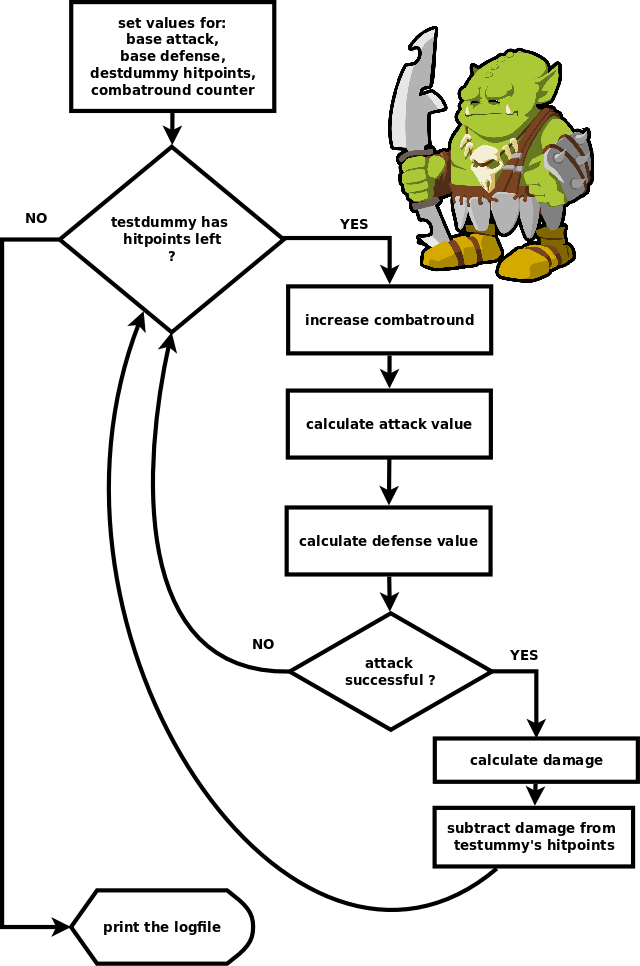
\includegraphics{goblindice001.png}
\end{flushright}\end{figure}

Imagine a young goblin named ``Grunty''. He dreams of being a fearsome warrior one day. However, at the moment, he is rather unskilled and barely capable of handling a weapon. Grunty goes to the training place fighting against a wooden testdummy.

Handling a weapon is no easy task, and Grunty will, despite his best efforts, not always land a blow. Sometimes he will miss.

Independent of the graphical representation (there is none yet), some combat mechanics must be formulated so that the computer can emulate a fight.

Let us assume that -like a \code{pen \& paper} role player- Grunty has a low basic chance of hitting the testdummy while swinging his weapon. We express that as a low integer (whole) like  3. A more skilled warrior would have an higher attack value. A line of python code saying just that would look like:

\begin{Verbatim}[commandchars=\\\{\}]
\PYG{n}{grunty\PYGZus{}base\PYGZus{}attack} \PYG{o}{=} \PYG{l+m+mi}{3}
\end{Verbatim}

The part left of the equal sign is called a \code{variable} (because some time in the future hopefully Gruntys attack value will increase) and the part right from the equal sign is called a value. In this case, an \code{integer} value because we use whole numbers (no decimal point). Decimal numbers (like 0.3) are called \code{float} values. Note that in python, variable names can not include a space (python would think those are two different commands) and therefore an underscore \code{\_} is used. It is also possible to use \emph{camelCase} like:  \code{gruntyAttack} instead. By convention, all variable names begin with a lowercase character.

But not every strike is the same for Grunty. Sometimes he has luck and performs a perfect attack, sometimes not. To reflect this variety, let us add some random values on top his base chance, to reflect the actual luck / skill / performance / difficulty of combat. To calculate the outcome of one single attack in a combat situation, some random value is added to the base attack value. In pen \& paper role playing games, the player has usually to throw two dice and add the number of eyes rolled to the base attack value.

\begin{Verbatim}[commandchars=\\\{\}]
\PYG{n}{attack\PYGZus{}value} \PYG{o}{=} \PYG{n}{grunty\PYGZus{}base\PYGZus{}attack} \PYG{o}{+} \PYG{n}{random\PYGZus{}integer\PYGZus{}value}
\end{Verbatim}

The resulting attack\_value is now hopefully greater than the base attack value. Let it compare to a similar calculated defense value to see if Grunty scored a hit.

Grunty is fighting against a wooden, unmovable testdummy. The testdummy is very easy to hit: We give it a extreme low defense value of 1, reflecting instrinct defense abilitys like diffictult-to-hit geometry and shape.

\begin{Verbatim}[commandchars=\\\{\}]
\PYG{n}{base\PYGZus{}defense} \PYG{o}{=} \PYG{l+m+mi}{1}
\end{Verbatim}

In actual combat, sometimes even an heap of wood can get lucky... not by actual moving, but maybe the sun is in his rear, blending the attacker, maybe the wind and the rain work in his favor. So to calcualte actual combat performance, let us add some random value on top of the (low) base defense value, but less than for the attacker. Let's say only rolling one die is allowed to roll and added to the base defense.

\begin{Verbatim}[commandchars=\\\{\}]
\PYG{n}{defense\PYGZus{}value} \PYG{o}{=} \PYG{n}{base\PYGZus{}defense} \PYG{o}{+} \PYG{n}{random\PYGZus{}integer\PYGZus{}value}
\end{Verbatim}

The combat runs in several combat rounds:
In each combat round, the computer calculates the attack and defense values (using his random generator functions) and compares those two. If the attacking value is greater than the defending value, Grunty managed a hit on the testdummy. If both values are equal, Grunty manages a ``glancing blow'', a hit that does no damage. If the attack value is greater than the defense value, damage is calculated as an random number between 0 and 10. With dice, this could be calculated by rolling 2 dice and subtracting 2 from the sum of eyes.

The damage is then substracted from the ``Hitpoints'' (also an integer number) of the testdummy, and the whole process is reapeated until the testdummy has no hitpoints left.

The fresh, undamaged testdummy must start with an given number of hitpoints, say 200 hiptoints. Also it is interesting to know how many combat rounds Grunty needs to destroy the testdummy, so a combat round counter is needed and set to 0 (you will soon see why) before the game.

\begin{Verbatim}[commandchars=\\\{\}]
\PYG{n}{testudmmy\PYGZus{}hitpoints} \PYG{o}{=} \PYG{l+m+mi}{200}
\PYG{n}{combat\PYGZus{}round\PYGZus{}counter} \PYG{o}{=} \PYG{l+m+mi}{0}
\end{Verbatim}

If you have read the instructions above you have basically read a program (that is a set of instructions) and you could now simulate Gruntys combat performance by using those instructions, a pair of dice and paper and pen to keep track of combat rounds and hitpoints.

To let a computer do this task instead, a set of commands and concepts is necessary:
\begin{itemize}
\item {} 
\emph{Variables}: numbers that can have different values over time, like the testdummys hitpoints or the round counter

\item {} 
\emph{Operators} to compare two variables

\item {} 
\emph{Control structures}:
\begin{itemize}
\item {} 
a \emph{Conditional} \code{if} statement to decide what to do if the attack value is greater than the defense value

\item {} 
a \emph{Loop} to repeat the whole process as long as necessary

\end{itemize}

\item {} 
Some random generator \emph{functions}

\end{itemize}


\chapter{Code}
\label{goblindice001:code}

\section{prerequesites}
\label{goblindice001:prerequesites}\begin{itemize}
\item {} 
necessary:
\begin{itemize}
\item {} 
python3 installed

\item {} 
text editor can save python files ( like \emph{goblindice001.py})

\item {} 
python3 interpreter can launch saved python file.

\end{itemize}

\item {} 
recommended:
\begin{itemize}
\item {} 
python-friendly IDE like IDLE, Geany etc.

\item {} 
ability to read and type (blind typing) using the 10 finger system, instead of copy and paste

\item {} 
python shell to lookup commands

\item {} 
executing python with filename as parameter from the command line \emph{python3 goblindice001.py})

\end{itemize}

\end{itemize}


\section{source code}
\label{goblindice001:source-code}
\begin{Verbatim}[commandchars=\\\{\},numbers=left,firstnumber=1,stepnumber=1]
\PYG{l+s+sd}{\PYGZdq{}\PYGZdq{}\PYGZdq{}}
\PYG{l+s+sd}{Name:             goblindice001.py }

\PYG{l+s+sd}{Purpose:          teaching basic python: while, if, elif, else, +=}
\PYG{l+s+sd}{idea:             simple combat sim of one goblin against a test dummy}
\PYG{l+s+sd}{edit this code:   https://github.com/horstjens/ThePythonGameBook/}
\PYG{l+s+sd}{                  blob/master/python/goblindice/goblindice001.py}
\PYG{l+s+sd}{edit tutorial:    https://github.com/horstjens/ThePythonGameBook/}
\PYG{l+s+sd}{                  blob/master/goblindice001.rst                  }
\PYG{l+s+sd}{main project:     http://ThePythonGameBook.com}
\PYG{l+s+sd}{Author:           Horst JENS, horst.jens@spielend\PYGZhy{}programmieren.at}
\PYG{l+s+sd}{Licence:          gpl, see http://www.gnu.org/licenses/gpl.html}
\PYG{l+s+sd}{\PYGZdq{}\PYGZdq{}\PYGZdq{}}
\PYG{k+kn}{import} \PYG{n+nn}{random} 
 
\PYG{c}{\PYGZsh{} Grunty, the untrained goblin, has some attack skill}
\PYG{n}{grunty\PYGZus{}attack} \PYG{o}{=} \PYG{l+m+mi}{3}   \PYG{c}{\PYGZsh{} integer value }
 
\PYG{c}{\PYGZsh{} the wooden, unmovable testdummy has poor defense, but many hitpoints}
\PYG{n}{testdummy\PYGZus{}hitpoints} \PYG{o}{=} \PYG{l+m+mi}{200} \PYG{c}{\PYGZsh{} integer value}
\PYG{n}{testdummy\PYGZus{}defense} \PYG{o}{=} \PYG{l+m+mi}{1}
 
\PYG{n}{logfile} \PYG{o}{=} \PYG{l+s}{\PYGZdq{}}\PYG{l+s}{ Grunty vs. the wooden testdummy}\PYG{l+s}{\PYGZdq{}}   \PYG{c}{\PYGZsh{} string}
\PYG{n}{combatround} \PYG{o}{=} \PYG{l+m+mi}{0} 
 
\PYG{k}{while} \PYG{n}{testdummy\PYGZus{}hitpoints} \PYG{o}{\PYGZgt{}} \PYG{l+m+mi}{0}\PYG{p}{:}
    \PYG{n}{combatround} \PYG{o}{+}\PYG{o}{=} \PYG{l+m+mi}{1}        \PYG{c}{\PYGZsh{} the same as: combatround = combatround +1}
    \PYG{n}{logfile} \PYG{o}{+}\PYG{o}{=} \PYG{l+s}{\PYGZdq{}}\PYG{l+s+se}{\PYGZbs{}n}\PYG{l+s}{*** Round: }\PYG{l+s}{\PYGZdq{}} \PYG{o}{+} \PYG{n+nb}{str}\PYG{p}{(}\PYG{n}{combatround}\PYG{p}{)} \PYG{o}{+} \PYG{l+s}{\PYGZdq{}}\PYG{l+s}{ ***}\PYG{l+s}{\PYGZdq{}} \PYG{c}{\PYGZsh{} \PYGZbs{}n new line}
    \PYG{n}{logfile} \PYG{o}{+}\PYG{o}{=} \PYG{l+s}{\PYGZdq{}}\PYG{l+s}{, target has \PYGZob{}\PYGZcb{} hitpoints}\PYG{l+s}{\PYGZdq{}}\PYG{o}{.}\PYG{n}{format}\PYG{p}{(}\PYG{n}{testdummy\PYGZus{}hitpoints}\PYG{p}{)}
    \PYG{n}{attack}\PYG{o}{=} \PYG{n}{grunty\PYGZus{}attack} \PYG{o}{+} \PYG{n}{random}\PYG{o}{.}\PYG{n}{randint}\PYG{p}{(}\PYG{l+m+mi}{1}\PYG{p}{,}\PYG{l+m+mi}{6}\PYG{p}{)}\PYG{o}{+}\PYG{n}{random}\PYG{o}{.}\PYG{n}{randint}\PYG{p}{(}\PYG{l+m+mi}{1}\PYG{p}{,}\PYG{l+m+mi}{6}\PYG{p}{)}
    \PYG{n}{defense} \PYG{o}{=} \PYG{n}{testdummy\PYGZus{}defense} \PYG{o}{+} \PYG{n}{random}\PYG{o}{.}\PYG{n}{randint}\PYG{p}{(}\PYG{l+m+mi}{1}\PYG{p}{,}\PYG{l+m+mi}{6}\PYG{p}{)} \PYG{c}{\PYGZsh{} roll one die}
    \PYG{k}{if} \PYG{n}{attack} \PYG{o}{\PYGZgt{}} \PYG{n}{defense}\PYG{p}{:} \PYG{c}{\PYGZsh{} did Grunty hit the testdummy ?}
        \PYG{n}{logfile} \PYG{o}{+}\PYG{o}{=} \PYG{l+s}{\PYGZdq{}}\PYG{l+s+se}{\PYGZbs{}n}\PYG{l+s}{Smack! Grunty hits his target with a most }\PYG{l+s}{\PYGZdq{}}
        \PYG{n}{logfile} \PYG{o}{+}\PYG{o}{=} \PYG{l+s}{\PYGZdq{}}\PYG{l+s}{skilled attack: \PYGZob{}\PYGZcb{} \PYGZgt{} \PYGZob{}\PYGZcb{}}\PYG{l+s}{\PYGZdq{}}\PYG{o}{.}\PYG{n}{format}\PYG{p}{(}\PYG{n}{attack}\PYG{p}{,} \PYG{n}{defense}\PYG{p}{)}
        \PYG{n}{damage} \PYG{o}{=} \PYG{n}{random}\PYG{o}{.}\PYG{n}{randint}\PYG{p}{(}\PYG{l+m+mi}{1}\PYG{p}{,}\PYG{l+m+mi}{6}\PYG{p}{)}\PYG{o}{+}\PYG{n}{random}\PYG{o}{.}\PYG{n}{randint}\PYG{p}{(}\PYG{l+m+mi}{1}\PYG{p}{,}\PYG{l+m+mi}{6}\PYG{p}{)}\PYG{o}{\PYGZhy{}}\PYG{l+m+mi}{2} \PYG{c}{\PYGZsh{} 0\PYGZhy{}10 damage}
        \PYG{n}{testdummy\PYGZus{}hitpoints} \PYG{o}{\PYGZhy{}}\PYG{o}{=} \PYG{n}{damage}   \PYG{c}{\PYGZsh{} subtract damage from hitpoints}
        \PYG{n}{logfile} \PYG{o}{+}\PYG{o}{=} \PYG{l+s}{\PYGZdq{}}\PYG{l+s+se}{\PYGZbs{}n}\PYG{l+s}{...and inflicts \PYGZob{}\PYGZcb{} damage!}\PYG{l+s}{\PYGZdq{}}\PYG{o}{.}\PYG{n}{format}\PYG{p}{(}\PYG{n}{damage}\PYG{p}{)}
    \PYG{k}{elif} \PYG{n}{attack} \PYG{o}{==} \PYG{n}{defense}\PYG{p}{:}
        \PYG{n}{logfile} \PYG{o}{+}\PYG{o}{=} \PYG{l+s}{\PYGZdq{}}\PYG{l+s+se}{\PYGZbs{}n}\PYG{l+s}{Grunty manages to nearly hit the target, but }\PYG{l+s}{\PYGZdq{}}
        \PYG{n}{logfile} \PYG{o}{+}\PYG{o}{=} \PYG{l+s}{\PYGZdq{}}\PYG{l+s}{he makes no damage \PYGZob{}0\PYGZcb{} = \PYGZob{}0\PYGZcb{}}\PYG{l+s}{\PYGZdq{}}\PYG{o}{.}\PYG{n}{format}\PYG{p}{(}\PYG{n}{attack}\PYG{p}{)}
    \PYG{k}{else}\PYG{p}{:}
        \PYG{n}{logfile} \PYG{o}{+}\PYG{o}{=} \PYG{l+s}{\PYGZdq{}}\PYG{l+s+se}{\PYGZbs{}n}\PYG{l+s}{ Oh no! Grunty does not even hit his target }\PYG{l+s}{\PYGZdq{}}
        \PYG{n}{logfile} \PYG{o}{+}\PYG{o}{=}  \PYG{l+s}{\PYGZdq{}}\PYG{l+s}{\PYGZob{}\PYGZcb{} \PYGZlt{} \PYGZob{}\PYGZcb{}}\PYG{l+s}{\PYGZdq{}}\PYG{o}{.}\PYG{n}{format}\PYG{p}{(}\PYG{n}{attack}\PYG{p}{,} \PYG{n}{defense}\PYG{p}{)}
\PYG{n}{logfile} \PYG{o}{+}\PYG{o}{=} \PYG{l+s}{\PYGZdq{}}\PYG{l+s+se}{\PYGZbs{}n}\PYG{l+s}{\PYGZdq{}} \PYG{o}{+} \PYG{l+s}{\PYGZdq{}}\PYG{l+s}{\PYGZhy{} }\PYG{l+s}{\PYGZdq{}} \PYG{o}{*} \PYG{l+m+mi}{20} \PYG{c}{\PYGZsh{} make a dashed line by multiplying a string}
\PYG{n}{logfile} \PYG{o}{+}\PYG{o}{=} \PYG{l+s}{\PYGZdq{}}\PYG{l+s+se}{\PYGZbs{}n}\PYG{l+s}{Victory for Grunty after \PYGZob{}\PYGZcb{} rounds}\PYG{l+s}{\PYGZdq{}}\PYG{o}{.}\PYG{n}{format}\PYG{p}{(}\PYG{n}{combatround}\PYG{p}{)}

\PYG{k}{print}\PYG{p}{(}\PYG{n}{logfile}\PYG{p}{)}
\end{Verbatim}


\section{output}
\label{goblindice001:output}
Some example output:

\begin{Verbatim}[commandchars=\\\{\}]
*** Round: 22 ***, target has 104 hitpoints
 Oh no! Grunty does not even hit his target 5 \PYGZlt{} 9
*** Round: 23 ***, target has 104 hitpoints
Grunty manages to nearly hit the target, but he makes no damage 9 = 9
*** Round: 24 ***, target has 104 hitpoints
Smack! Grunty hits his target with a most skilled attack: 6 \PYGZgt{} 4
...and inflicts 2 damage!
*** Round: 25 ***, target has 102 hitpoints
Oh no! Grunty does not even hit his target 6 \PYGZlt{} 9
\end{Verbatim}


\section{code discussion}
\label{goblindice001:code-discussion}
Some elements in this code may need explaining:

\begin{tabulary}{\linewidth}{|L|L|L|}
\hline
\textsf{\relax 
line number
} & \textsf{\relax 
term
} & \textsf{\relax 
explanation
}\\
\hline
1 - 13
 & 
\href{http://docs.python.org/glossary.html\#term-docstring}{\emph{docstring}}
 & 
Some multi-line text \emph{string} insinde triple-quotes \code{"""}. If a docstring is the first statement in a file it is automatically stored in the gloabel variable \code{\_\_doc\_\_}. Docstrings are interpreted by python as something interested for humans only, like a \emph{comment}. Docstrings are not necessary, but nice to have.
\\
\hline
14
 & 
\code{import random}
 & 
To make use of any \emph{functon} in pythons random module, it is necessary to import this module first. Later in this code functions of the random module will use the prefix \code{random.}.
\\
\hline
16
 & 
\code{comment}
 & 
Everything behind a \code{\#} sign in python is a comment. Comments are useful for human eyes only and always ignored by Python.
\\
\hline
17
 & 
\code{assign}, \code{inline comment}
 & 
The value of 3 is assigned to the variable \code{grunty\_attack}. (You best read it from right to left).  Note that the part right from the \code{\#} sign is also a comment.
\\
\hline
26
 & 
\code{loop}, \code{expresssion}
 & 
The \code{while} \code{keyword} indicates, together with the colon at the end of this line, the beginning of an \code{indented code block}. This code block is reapeated as long as the \code{expression{}`{}`right from {}`{}`while{}`{}`remains {}`{}`True}.
\\
\hline
27
 & 
\code{increment}
 & 
The value of the the \code{variable} \code{combatround} is incremented by 1. Because this is made even before some combat values are calculated, \code{combatround} was set to 0 before the while loop.
\\
\hline
28
 & 
\code{strings and numbers}
 & 
Another textstring is appended to the textstring variable \code{logfile}. The starting new line sign (\code{\textbackslash{}n}) is a so called \code{escaped character}. Because \code{combatround} is of type integer, it can \emph{not} be appended to the textstring \code{logfile}. Therefore, `'combatround'' must first be converted into a string using the \code{str()} function.
\\
\hline
29
 & 
\code{format mini language}
 & 
Using Format String Syntax instead of the \code{str} function, the curly brackets are replaced by python with the expression inside the round brackets of \code{.format()}. See \href{https://docs.python.org/2/library/string.html}{https://docs.python.org/2/library/string.html}
\\
\hline
30
 & 
\code{random.randint()}
 & 
The \code{random.randint()} function generates a (nearly) random integer between (including) the first (lower) and the second (higher) number in the round brackets. Writing instead \code{random.randint(1,6)*2} or \code{random.randint(2,12)} would be similar, but not the same. See next page for more on this topic.
\\
\hline
32
 & 
\code{conditional}, \code{if}
 & 
Like the \code{while} keyword, the \code{if} keyword need an expression and a colon and is followed by an \code{idented code block}. This code block will only be executed if the  \code{expression} is \code{True}. Note that you can write an inline-comment after the colon with the \code{\#} sign. For python, the comment is ignored and the line ends with the colon.
\\
\hline
33 - 34
 & 
\code{strings}
 & 
Note that the string in line 33 ends with an space and the string in line 34 does not begin with a new line. In fact, line 33 and line 34 can be written in lone (very long) line. In this case, two seperate lines were written for layout reasons, to make no code line longer than 72 characters. See \href{http://legacy.python.org/dev/peps/pep-0008/}{http://legacy.python.org/dev/peps/pep-0008/}
\\
\hline
34
 & 
\code{format mini language}
 & 
The first pair of curly brackets get replaced by the first value inside \code{.format()}, the second pair of curly brackets get replaced by the second value inside \code{.format()} and so on.
\\
\hline
35
 & 
\code{random.randint())}
 & 
Here, {\color{red}\bfseries{}{}`{}`}random.randint(2,12) could have be used instead, and would have resulted similar, bot not exact the same distribution of random values as this formular. See next page for more details.
\\
\hline
36
 & 
\code{decrement}
 & 
Like the increment, this line could have been written as: \code{testdummy\_hitpoints -= testdummy\_hitpoints - damage}. But why type more than necessary?
\\
\hline\end{tabulary}


pause

\begin{tabulary}{\linewidth}{|L|L|L|}
\hline
\textsf{\relax 
line number
} & \textsf{\relax 
term
} & \textsf{\relax 
explanation
}\\
\hline
38
 & 
\code{elif}
 & 
Each \code{if} code block can have many (including none) \code{elif} code blocks. Like the \code{if} keyword, the \code{indented code block} after elif will only be executed if the \code{expression} was False for all previous \code{elif} expressions as well as for the initial \code{if} and only if the actual expression (right of \code{elif}) is \code{True}.
\\
\hline
38
 & 
\code{equal test}
 & 
Please note that the \emph{==} operator is used to \emph{test for equality}. The \emph{=} operator assigns values.
\\
\hline
40
 & 
\code{format mini language}
 & 
A special trick using \code{.format()}: When you have one variable at several places inside a string, like in this case, you can use their number inside the curly bracket. Python always start counting with 0, so the first variable in the round brackets is referred as \code{\{0\}}, the second variable as \code{\{1\}} and so on.
\\
\hline
41
 & 
\code{else}
 & 
If the \code{if} and all \code{elif} expressions are \code{False}, the \code{idented code block} behind the \code{else:} keyword is executed. The \code{else:} keyword itself is optional and need no expression behind it.
\\
\hline
44
 & 
\code{indentation}
 & 
This line is \emph{outside} the \code{while block} ! Take a close look at the previous line with the same indentation: It's line 26. That means that this line will only executed if the expression in line 26 becomes \code{False}
\\
\hline
46
 & 
\code{empty line}
 & 
There is no specific reason to let this line empty: it's just to have the code pretty layouted. Python ignores empty lines.
\\
\hline
47
 & 
\code{print()}
 & 
The \code{print()} keyword can output any variable to the screen. Note that since python version 3, \code{print} need round brackets.
\\
\hline\end{tabulary}


next page: functions !


\chapter{Goblin dice tutorial}
\label{goblindice_start:goblin-dice-tutorial}
This is the goblin dice tutorial starting page.

This document is meant to give a tutorial-like overview of all common tasks
while using Sphinx.

The green arrows designate ``more info'' links leading to advanced sections about
the described task.

let us start :


\section{boring welcome headline}
\label{goblindice_start:boring-welcome-headline}
with some not necessary text below it


\section{second boring sub-headline}
\label{goblindice_start:second-boring-sub-headline}
also with non-relevant text


\chapter{Indices and tables}
\label{index:indices-and-tables}\begin{itemize}
\item {} 
\emph{genindex}

\item {} 
\emph{modindex}

\item {} 
\emph{search}

\end{itemize}



\renewcommand{\indexname}{Index}
\printindex
\end{document}
